% =====================================================================
%  Aprendizaje No Supervisado — Sesión 5: Agrupamiento por densidad y espectral
%  Unidad 1: Algoritmos de agrupamiento
%  Compilar con: latexmk -pdf Sesion5-Densidad_Espectral.tex
%  Figuras: python3 figuras/generar_figuras.py
%  El laboratorio está en Laboratorio.tex (se incluye al final con \input)
% =====================================================================
\documentclass[aspectratio=169,11pt]{beamer}

\usepackage[utf8]{inputenc}
\usepackage[T1]{fontenc}
\usepackage[spanish,es-noshorthands,es-nodecimaldot]{babel}
\usepackage{amsmath,amssymb,bm}
\usepackage{booktabs,array}
\usepackage{listings}
\usepackage{tikz}
\usetikzlibrary{positioning,arrows.meta}
\graphicspath{{figuras/}}
\tikzset{caja/.style={draw=azul,fill=azul!10,rounded corners,align=center,font=\small,
  minimum height=9mm}}

% ---------- Tema (común a las presentaciones del curso) ----------
\usetheme{Madrid}
\usefonttheme{professionalfonts}
\definecolor{marino}{HTML}{1F3864}
\definecolor{azul}{HTML}{2E75B6}
\definecolor{naranja}{HTML}{E07B22}
\definecolor{verde}{HTML}{5B9A3C}
\definecolor{fondocod}{HTML}{F4F6F9}
\setbeamercolor{palette primary}{bg=marino,fg=white}
\setbeamercolor{palette secondary}{bg=azul,fg=white}
\setbeamercolor{palette tertiary}{bg=marino,fg=white}
\setbeamercolor{frametitle}{bg=marino,fg=white}
\setbeamercolor{title}{bg=marino,fg=white}
\setbeamercolor{structure}{fg=azul}
\setbeamercolor{block title}{bg=azul,fg=white}
\setbeamercolor{block body}{bg=azul!8}
\setbeamercolor{block title alerted}{bg=naranja,fg=white}
\setbeamercolor{block body alerted}{bg=naranja!10}
\setbeamercolor{block title example}{bg=verde,fg=white}
\setbeamercolor{block body example}{bg=verde!10}
\setbeamercolor{alerted text}{fg=naranja}
\setbeamertemplate{navigation symbols}{}
\setbeamertemplate{itemize items}[circle]
\setbeamertemplate{blocks}[rounded][shadow=false]

\AtBeginSection[]{
  \begin{frame}
    \vfill\centering
    \begin{beamercolorbox}[sep=12pt,center,rounded=true]{title}
      \usebeamerfont{title}\insertsectionhead
    \end{beamercolorbox}
    \vfill
  \end{frame}
}

\lstdefinestyle{py}{
  language=Python, basicstyle=\ttfamily\scriptsize,
  keywordstyle=\color{marino}\bfseries, commentstyle=\color{gray}\itshape,
  stringstyle=\color{naranja}, backgroundcolor=\color{fondocod},
  frame=single, rulecolor=\color{azul!40}, showstringspaces=false,
  columns=fullflexible, breaklines=true, xleftmargin=4pt, xrightmargin=4pt,
  literate={á}{{\'a}}1 {é}{{\'e}}1 {í}{{\'i}}1 {ó}{{\'o}}1 {ú}{{\'u}}1 {ñ}{{\~n}}1
}
\lstset{style=py}

\newcommand{\R}{\mathbb{R}}
\newcommand{\x}{\bm{x}}
\newcommand{\muv}{\bm{\mu}}
\newcommand{\eps}{\varepsilon}

\title[Sesión 5: Densidad y espectral]{Sesión 5: Agrupamiento por densidad y espectral}
\subtitle{Aprendizaje No Supervisado --- Unidad 1: Algoritmos de agrupamiento}
\author[A. Espinosa Romero]{Arturo Espinosa Romero}
\institute[FMAT]{Maestría en Inteligencia Artificial \\ Facultad de Matemáticas}
\date{Sesión 5}

% =====================================================================
\begin{document}

\begin{frame}
  \titlepage
\end{frame}

\begin{frame}{Agenda de la sesión}
  \begin{columns}[T]
    \column{0.55\textwidth}
    \begin{enumerate}
      \item Grupos que no son convexos
      \item DBSCAN: núcleo, frontera y ruido
      \item Densidad variable: OPTICS y HDBSCAN
      \item Agrupamiento espectral: grafo y laplaciano
      \item Laboratorio: DBSCAN, HDBSCAN y espectral en formas no convexas
    \end{enumerate}
    \column{0.4\textwidth}
    \begin{block}{Al terminar podrás}
      \begin{itemize}
        \item Explicar qué es un grupo definido por densidad
        \item Elegir $\eps$ y \texttt{min\_samples}
        \item Reconocer cuándo hace falta HDBSCAN
        \item Explicar por qué el laplaciano separa grupos
      \end{itemize}
    \end{block}
  \end{columns}
\end{frame}

% =====================================================================
\section{Grupos que no son convexos}
% =====================================================================

\begin{frame}{Problema detonador: lunas y círculos}
  \begin{columns}[c]
    \column{0.5\textwidth}
    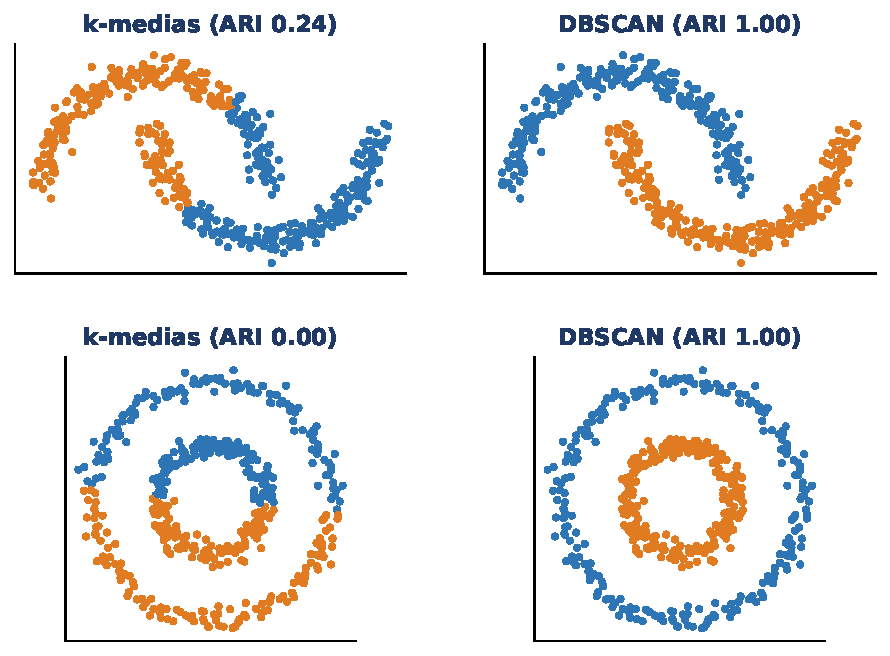
\includegraphics[width=0.92\textwidth]{detonador}
    \column{0.48\textwidth}
    \begin{itemize}
      \item k-medias, Ward y GMM suponen grupos \textbf{convexos}.
      \item Con dos lunas entrelazadas, k-medias corta cada luna (ARI 0.24); con dos círculos
            concéntricos, parte el plano por la mitad (ARI 0.00).
      \item DBSCAN sigue las zonas de alta densidad y recupera los grupos (ARI 1.00).
    \end{itemize}
    \begin{block}{Otra definición de grupo}
      Un grupo es una región \alert{densa} separada de otras por regiones de baja densidad,
      sin importar su forma.
    \end{block}
  \end{columns}
\end{frame}

% =====================================================================
\section{DBSCAN}
% =====================================================================

\begin{frame}{Densidad con dos parámetros}
  \textbf{DBSCAN} (Ester, Kriegel, Sander y Xu, 1996): \emph{Density-Based Spatial Clustering of
  Applications with Noise}.
  \vspace{4pt}
  \begin{itemize}
    \item $\eps$-vecindad de un punto: $N_\eps(\x) = \{\bm{y} : \|\x - \bm{y}\| \le \eps\}$.
    \item \texttt{min\_samples} $= m$: cuántos puntos debe tener la vecindad para considerarla densa
          (en scikit-learn cuenta el propio punto).
  \end{itemize}
  \vspace{4pt}
  \begin{columns}[T]
    \column{0.32\textwidth}
    \begin{block}{Núcleo}
      $|N_\eps(\x)| \ge m$: el punto está en una zona densa.
    \end{block}
    \column{0.32\textwidth}
    \begin{block}{Frontera}
      No es núcleo, pero está en la vecindad de algún núcleo.
    \end{block}
    \column{0.32\textwidth}
    \begin{alertblock}{Ruido}
      No es núcleo ni está en la vecindad de un núcleo.
    \end{alertblock}
  \end{columns}
  \vspace{6pt}
  Un \textbf{grupo} es un conjunto máximo de núcleos conectados entre sí (cada uno en la vecindad
  del siguiente), más los puntos frontera que los rodean.
\end{frame}

\begin{frame}{Núcleo, frontera y ruido}
  \begin{columns}[c]
    \column{0.52\textwidth}
    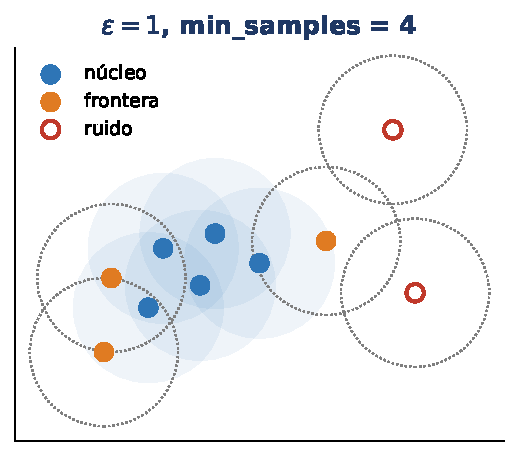
\includegraphics[width=\textwidth]{dbscan_puntos}
    \column{0.46\textwidth}
    \small
    \begin{itemize}
      \item Círculos: vecindades de radio $\eps$. Sombreadas, las de los núcleos.
      \item 5 núcleos forman un grupo; 3 puntos frontera se unen a él.
      \item Los 2 puntos de la derecha tienen vecinos, pero ninguno es núcleo: son ruido.
      \item Un punto frontera puede estar cerca de núcleos de dos grupos: se asigna al primero
            que lo alcance (depende del orden de los datos).
    \end{itemize}
  \end{columns}
\end{frame}

\begin{frame}{Ejemplo resuelto en una dimensión}
  Datos $\{1, 2, 3, 4, 8, 9, 15\}$, \ $\eps = 1.5$, \ \texttt{min\_samples} $= 3$.
  \vspace{6pt}
  \centering
  \begin{tikzpicture}[x=7mm]
    \draw[->, gray] (0,0) -- (16,0);
    \foreach \v in {0,2,4,...,16} \node[below, gray, font=\scriptsize] at (\v,-0.1) {\v};
    \foreach \v in {2,3} \fill[azul] (\v,0) circle (4pt);
    \foreach \v in {1,4} \fill[naranja] (\v,0) circle (4pt);
    \foreach \v in {8,9,15} \draw[red!70!black, thick, fill=white] (\v,0) circle (4pt);
    \draw[azul, thick] (0.8,0.35) -- (4.2,0.35) node[midway, above, font=\small] {grupo 1};
  \end{tikzpicture}
  \vspace{6pt}
  \small
  \begin{tabular}{@{}lccccccc@{}}
    \toprule
    Punto & 1 & 2 & 3 & 4 & 8 & 9 & 15\\
    Vecinos a distancia $\le 1.5$ (incluido él) & 1, 2 & 1, 2, 3 & 2, 3, 4 & 3, 4 & 8, 9 & 8, 9 & 15\\
    Tamaño de la vecindad & 2 & 3 & 3 & 2 & 2 & 2 & 1\\
    Tipo & \textcolor{naranja}{frontera} & \textcolor{azul}{núcleo} & \textcolor{azul}{núcleo}
         & \textcolor{naranja}{frontera} & ruido & ruido & ruido\\
    \bottomrule
  \end{tabular}
  \vspace{6pt}
  \begin{itemize}
    \item 8 y 9 están juntos, pero dos puntos no alcanzan \texttt{min\_samples} $= 3$: son ruido, no un grupo.
    \item El número de grupos no se fija: sale de los datos y de $(\eps, m)$.
  \end{itemize}
\end{frame}

\begin{frame}{Cómo elegir $\eps$: la gráfica de k-distancia}
  \begin{columns}[c]
    \column{0.5\textwidth}
    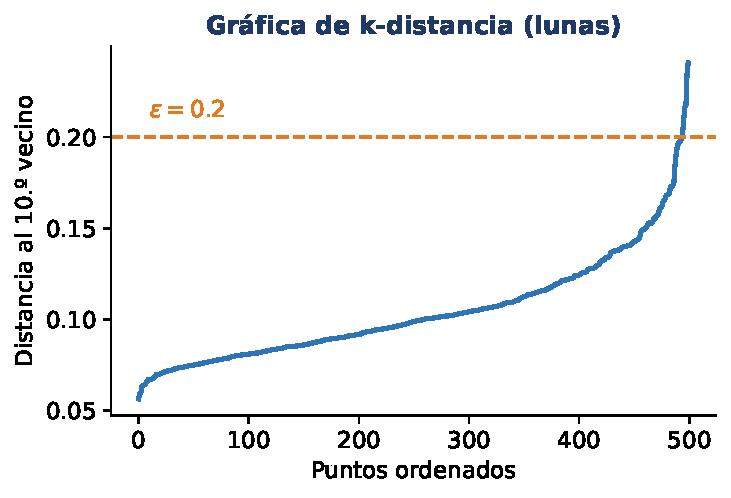
\includegraphics[width=\textwidth]{k_distancia}
    \column{0.48\textwidth}
    \small
    \begin{enumerate}
      \item Elegir \texttt{min\_samples} $=m$. Regla práctica: $m \ge d+1$; con ruido, $m \approx 2d$ o más.
      \item Calcular para cada punto la distancia a su $m$-ésimo vecino.
      \item Ordenarlas: los puntos de los grupos tienen distancias pequeñas; el ruido, grandes.
      \item Elegir $\eps$ en el ``codo'' donde la curva sube.
    \end{enumerate}
    Aquí, con $m=10$, el codo está cerca de $\eps = 0.2$.
  \end{columns}
\end{frame}

\begin{frame}{El efecto de $\eps$}
  \centering
  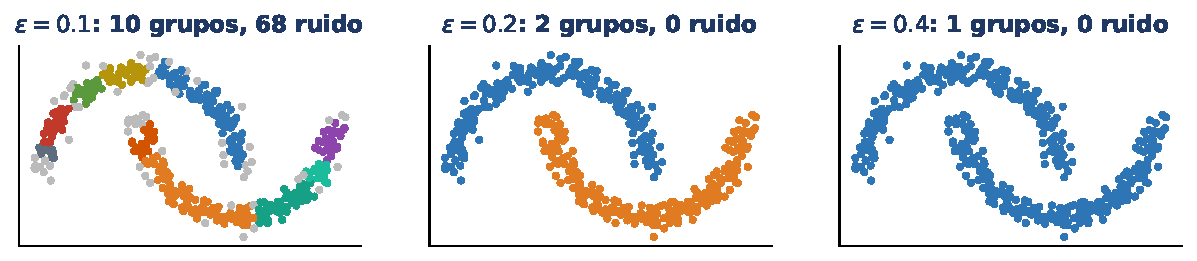
\includegraphics[width=0.95\textwidth]{dbscan_eps}
  \begin{itemize}
    \item $\eps$ pequeño: pocos núcleos; las lunas se rompen en fragmentos y mucho ruido.
    \item $\eps$ grande: las vecindades cruzan el hueco entre las lunas y todo se une en un grupo.
    \item Entre ambos extremos hay un intervalo de valores que funciona (aquí, 0.2 a 0.3).
  \end{itemize}
\end{frame}

\begin{frame}{DBSCAN: balance}
  \begin{columns}[T]
    \column{0.48\textwidth}
    \begin{exampleblock}{Ventajas}
      \begin{itemize}
        \item No hay que fijar el número de grupos.
        \item Grupos de cualquier forma.
        \item Detecta ruido explícitamente (etiqueta $-1$).
        \item Determinista para núcleos y ruido.
        \item $O(n \log n)$ con un índice espacial en dimensión baja; $O(n^2)$ en el peor caso.
      \end{itemize}
    \end{exampleblock}
    \column{0.48\textwidth}
    \begin{alertblock}{Limitaciones}
      \begin{itemize}
        \item Un solo $\eps$ para todo el espacio: falla si los grupos tienen
              \textbf{densidades distintas}.
        \item Sensible a la escala: hay que estandarizar si las variables tienen unidades distintas.
        \item En dimensión alta las distancias se parecen entre sí y elegir $\eps$ es difícil.
      \end{itemize}
    \end{alertblock}
  \end{columns}
\end{frame}

% =====================================================================
\section{Densidad variable: OPTICS y HDBSCAN}
% =====================================================================

\begin{frame}{Un $\eps$ no sirve para todos los grupos}
  \centering
  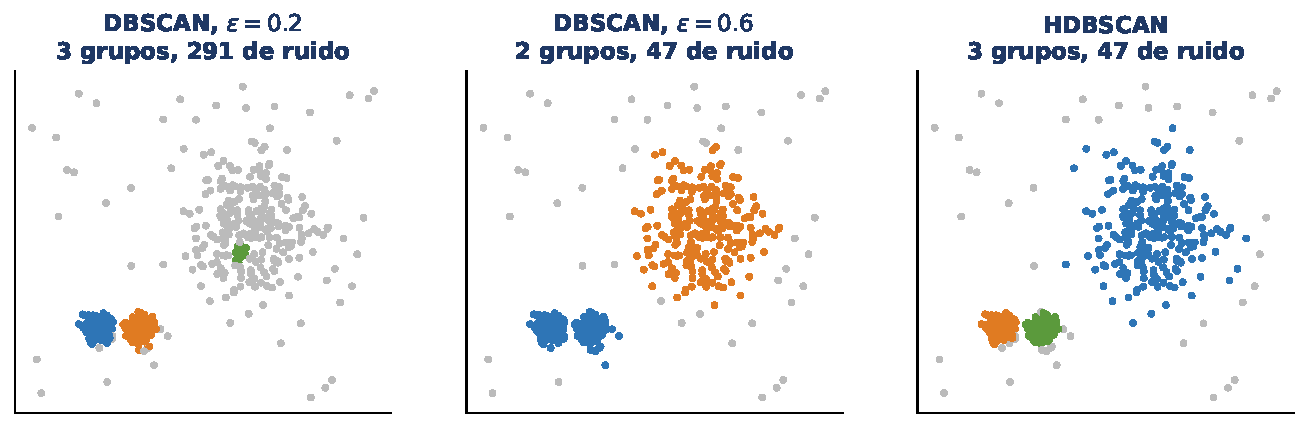
\includegraphics[width=0.95\textwidth]{densidad_variable}
  \begin{itemize}
    \item Dos grupos densos y pegados, uno disperso, y 50 puntos de ruido uniforme.
    \item $\eps=0.2$ separa los densos, pero 236 de los 250 puntos del disperso quedan como ruido.
    \item $\eps=0.6$ recupera el disperso, pero une los dos densos en un grupo.
    \item HDBSCAN encuentra los tres grupos sin elegir $\eps$.
  \end{itemize}
\end{frame}

\begin{frame}{Distancia de núcleo y alcanzabilidad}
  Las dos ideas en que se basan OPTICS y HDBSCAN:
  \begin{itemize}
    \item \textbf{Distancia de núcleo}: $\operatorname{core}_m(\x)$ = distancia de $\x$ a su
          $m$-ésimo vecino. Es el $\eps$ más pequeño con el que $\x$ sería núcleo;
          pequeña en zonas densas.
    \item \textbf{Distancia de alcanzabilidad} de $\bm{y}$ desde $\x$:
          $\max\{\operatorname{core}_m(\x),\ \|\x - \bm{y}\|\}$.
    \item \textbf{Distancia de alcanzabilidad mutua} (HDBSCAN):
          \[
            d_{\text{mreach}}(\x, \bm{y}) = \max\{\operatorname{core}_m(\x),\ \operatorname{core}_m(\bm{y}),\ \|\x - \bm{y}\|\}.
          \]
  \end{itemize}
  \vspace{4pt}
  \begin{block}{Efecto}
    En zonas densas no cambia las distancias; en zonas dispersas las agranda. Los puntos aislados
    quedan lejos de todos, y es fácil separarlos como ruido.
  \end{block}
\end{frame}

\begin{frame}{OPTICS: todos los $\eps$ a la vez}
  \centering
  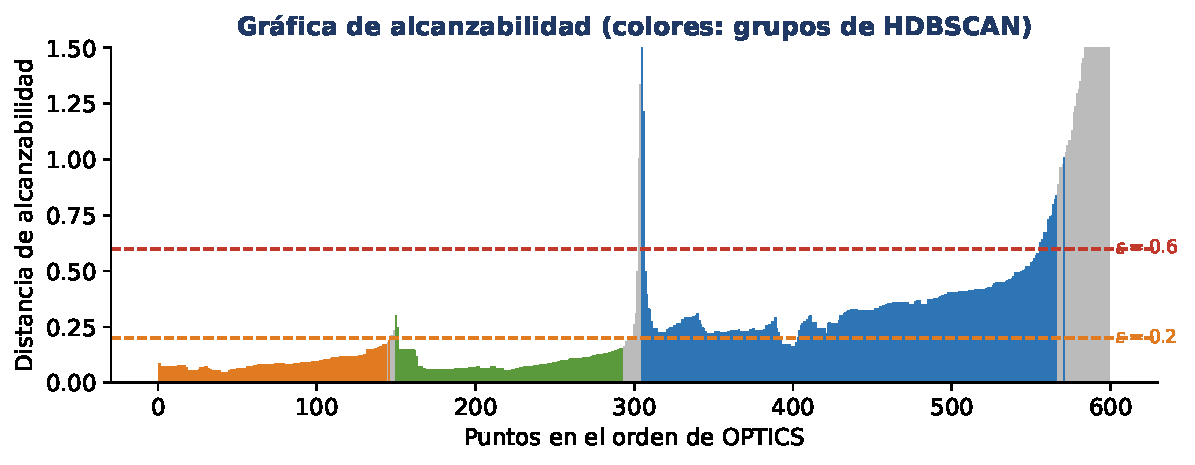
\includegraphics[width=0.78\textwidth]{optics_alcanzabilidad}
  \begin{itemize}
    \item OPTICS recorre los puntos yendo siempre al más alcanzable y grafica su alcanzabilidad.
    \item Cada \textbf{valle} es un grupo; su profundidad indica su densidad. Los dos grupos densos
          están muy abajo; el disperso, más arriba.
    \item Cortar la gráfica a la altura $\eps$ equivale a DBSCAN con ese $\eps$: ninguna línea
          horizontal separa los tres valles a la vez.
  \end{itemize}
\end{frame}

\begin{frame}{HDBSCAN: la jerarquía de densidad}
  \textbf{HDBSCAN} (Campello, Moulavi y Sander, 2013) combina DBSCAN con el agrupamiento jerárquico:
  \begin{enumerate}
    \item Calcular la distancia de alcanzabilidad mutua con $m$ = \texttt{min\_samples}.
    \item Construir el árbol de expansión mínima con esa distancia y, de él, la jerarquía de enlace
          simple (Sesión 3). Cortarla a la altura $\eps$ da el resultado de DBSCAN con ese $\eps$ (sin puntos frontera).
    \item \textbf{Condensar} el árbol: una división sólo cuenta si los dos lados tienen al menos
          \texttt{min\_cluster\_size} puntos; si no, se dice que el grupo ``pierde puntos''.
    \item Elegir los grupos más \textbf{estables}: los que persisten en un intervalo amplio de densidades.
  \end{enumerate}
  \vspace{4pt}
  \begin{columns}[T]
    \column{0.48\textwidth}
    \begin{exampleblock}{Resultado}
      Cada grupo se elige a su propia escala de densidad; no hay $\eps$ global.
    \end{exampleblock}
    \column{0.48\textwidth}
    \begin{block}{Parámetro principal}
      \texttt{min\_cluster\_size}: el tamaño mínimo de un grupo. Es más fácil de razonar que $\eps$.
    \end{block}
  \end{columns}
\end{frame}

% =====================================================================
\section{Agrupamiento espectral}
% =====================================================================

\begin{frame}{Agrupar los nodos de un grafo}
  \begin{enumerate}
    \item \textbf{Grafo de similitud} $W$ ($n \times n$, simétrica):
      \begin{itemize}
        \item $k$ vecinos más cercanos: $w_{ij} = 1$ si $j$ es vecino de $i$ o viceversa;
        \item núcleo gaussiano: $w_{ij} = \exp(-\gamma \|\x_i - \x_j\|^2)$;
        \item $\eps$-vecindad: $w_{ij} = 1$ si $\|\x_i - \x_j\| \le \eps$.
      \end{itemize}
    \item \textbf{Grado} de cada nodo: $d_i = \sum_j w_{ij}$, \ $D = \operatorname{diag}(d_1,\dots,d_n)$.
    \item \textbf{Laplaciano}: $L = D - W$, o su versión normalizada
          $L_{sym} = I - D^{-1/2} W D^{-1/2}$.
  \end{enumerate}
  \vspace{4pt}
  \begin{block}{Idea}
    Un buen agrupamiento corta pocas aristas (o aristas de peso pequeño) entre grupos y deja grupos
    de tamaño razonable. Ese problema de corte (\emph{RatioCut}, \emph{NCut}) es NP-difícil;
    su relajación continua se resuelve con los vectores propios de $L$.
  \end{block}
\end{frame}

\begin{frame}{Por qué funciona el laplaciano}
  Para cualquier vector $\bm{f} \in \R^n$ (un valor por nodo):
  \[
    \bm{f}^\top L\, \bm{f} = \frac12 \sum_{i,j} w_{ij}\, (f_i - f_j)^2 \;\ge\; 0 .
  \]
  \begin{itemize}
    \item $\bm{f}^\top L \bm{f}$ es pequeño si los nodos conectados tienen valores parecidos.
    \item Si el grafo tiene $K$ \textbf{componentes conexas}, el valor propio 0 tiene multiplicidad $K$,
          y sus vectores propios son los indicadores de cada componente.
    \item Si los grupos están \emph{casi} desconectados, los $K$ primeros vectores propios
          son \emph{casi} indicadores: en ese espacio los grupos quedan separados y compactos.
  \end{itemize}
  \vspace{4pt}
  \begin{block}{Algoritmo (Ng, Jordan y Weiss, 2002)}
    \begin{enumerate}
      \item Construir $W$ y $L_{sym}$.
      \item Tomar los $K$ vectores propios de $L_{sym}$ con valores propios más pequeños: $U \in \R^{n\times K}$.
      \item Normalizar las filas de $U$ y agruparlas con k-medias.
    \end{enumerate}
  \end{block}
\end{frame}

\begin{frame}{Los círculos en el espacio espectral}
  \centering
  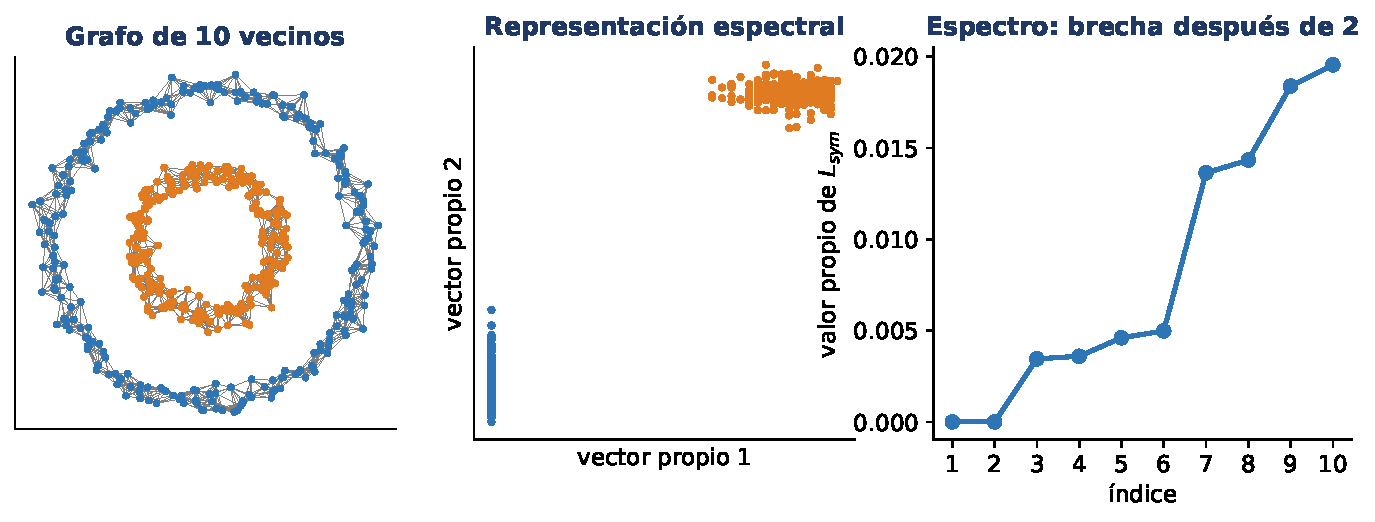
\includegraphics[width=0.88\textwidth]{espectral}
  \begin{itemize}
    \item El grafo de 10 vecinos no tiene aristas entre los círculos: tiene 2 componentes conexas.
    \item Por eso hay 2 valores propios iguales a 0, y en los dos primeros vectores propios cada
          círculo se reduce a un punto. k-medias los separa sin dificultad.
    \item La \textbf{brecha espectral} (salto después del $K$-ésimo valor propio) sugiere $K$.
  \end{itemize}
\end{frame}

\begin{frame}{Agrupamiento espectral: balance}
  \begin{columns}[T]
    \column{0.48\textwidth}
    \begin{exampleblock}{Ventajas}
      \begin{itemize}
        \item Grupos no convexos: sólo importa la conectividad del grafo.
        \item Sirve con cualquier similitud, incluso sin coordenadas (grafos, redes sociales).
        \item La brecha espectral orienta la elección de $K$.
      \end{itemize}
    \end{exampleblock}
    \column{0.48\textwidth}
    \begin{alertblock}{Limitaciones}
      \begin{itemize}
        \item Hay que fijar $K$.
        \item No detecta ruido: cada punto queda en algún grupo.
        \item Sensible a la construcción del grafo ($k$ o $\gamma$).
        \item Descomposición en valores propios: $O(n^3)$ con matrices densas;
              con grafos dispersos de vecinos, decenas de miles de puntos.
      \end{itemize}
    \end{alertblock}
  \end{columns}
\end{frame}

\begin{frame}{Resumen de los métodos de la Unidad 1}
  \centering
  \footnotesize
  \renewcommand{\arraystretch}{1.25}
  \begin{tabular}{@{}lccccc@{}}
    \toprule
    & \textbf{k-medias} & \textbf{GMM} & \textbf{Jerárquico} & \textbf{DBSCAN/HDBSCAN} & \textbf{Espectral}\\
    \midrule
    Fijar el número de grupos & sí & sí & al cortar & no & sí \\
    Grupos no convexos & no & no & enlace simple & sí & sí \\
    Densidades distintas & no & sí & no & sólo HDBSCAN & parcial \\
    Detecta ruido & no & no & no & sí & no \\
    Escala a $n$ & $10^6$ o más & $\sim 10^5$ & $\sim 10^4$ & $\sim 10^5$ & $\sim 10^4$ \\
    \bottomrule
  \end{tabular}
  \vspace{8pt}
  \begin{itemize}
    \item No hay un método mejor en general: depende de la forma, la densidad y el ruido de los grupos.
    \item En la Sesión 6 veremos cómo validar un agrupamiento cuando no hay etiquetas.
  \end{itemize}
\end{frame}

\begin{frame}[fragile]{Densidad y espectral en scikit-learn}
\begin{lstlisting}
from sklearn.cluster import DBSCAN, OPTICS, HDBSCAN, SpectralClustering

db = DBSCAN(eps=0.2, min_samples=10).fit(X)
db.labels_                    # -1 = ruido
db.core_sample_indices_       # indices de los puntos nucleo

op = OPTICS(min_samples=10).fit(X)
op.reachability_[op.ordering_]   # grafica de alcanzabilidad

hd = HDBSCAN(min_cluster_size=15).fit(X)   # min_samples = min_cluster_size por omision
hd.labels_, hd.probabilities_              # pertenencia: 0 = ruido, 1 = centro del grupo

sc = SpectralClustering(n_clusters=2, affinity="nearest_neighbors", n_neighbors=10,
                        random_state=0).fit(X)
sc.labels_
\end{lstlisting}
  {\small \texttt{HDBSCAN} está en scikit-learn desde la versión 1.3; antes, en el paquete \texttt{hdbscan}.}
\end{frame}

% =====================================================================
%  Laboratorio (para omitirlo de las láminas, comentar la línea siguiente)
% =====================================================================
%  Laboratorio de la Sesión 5: DBSCAN, HDBSCAN y agrupamiento espectral
%  en formas no convexas
%  Se incluye desde Sesion5-Densidad_Espectral.tex con % =====================================================================
%  Laboratorio de la Sesión 5: DBSCAN, HDBSCAN y agrupamiento espectral
%  en formas no convexas
%  Se incluye desde Sesion5-Densidad_Espectral.tex con % =====================================================================
%  Laboratorio de la Sesión 5: DBSCAN, HDBSCAN y agrupamiento espectral
%  en formas no convexas
%  Se incluye desde Sesion5-Densidad_Espectral.tex con \input{Laboratorio}
%  El mismo código, ejecutado, está en laboratorio_densidad_espectral.ipynb
% =====================================================================
\section{Laboratorio: densidad y espectral en formas no convexas}
% =====================================================================

\begin{frame}[fragile]{Paso 1: los datos}
\begin{lstlisting}
import numpy as np, pandas as pd
from sklearn.datasets import make_moons, make_circles, make_blobs
from sklearn.cluster import KMeans, DBSCAN, HDBSCAN, SpectralClustering
from sklearn.neighbors import NearestNeighbors
from sklearn.metrics import adjusted_rand_score

Xm, ym = make_moons(500, noise=0.07, random_state=0)
Xc, yc = make_circles(500, factor=0.45, noise=0.05, random_state=0)
Xb, yb = make_blobs([150, 150, 250], centers=[[0, 0], [1.3, 0], [4.5, 3]],
                    cluster_std=[0.2, 0.2, 1.0], random_state=0)
ruido = np.random.default_rng(0).uniform([-2, -2], [8, 7], (50, 2))
Xd, yd = np.r_[Xb, ruido], np.r_[yb, -np.ones(50, int)]   # el ruido tiene etiqueta -1
datos = {"Lunas": (Xm, ym), "Círculos": (Xc, yc), "Densidades": (Xd, yd)}
\end{lstlisting}
  {\small Las etiquetas verdaderas sólo se usan para evaluar con el ARI; el ruido cuenta como una clase más.}
\end{frame}

\begin{frame}{Paso 1: los tres conjuntos}
  \centering
  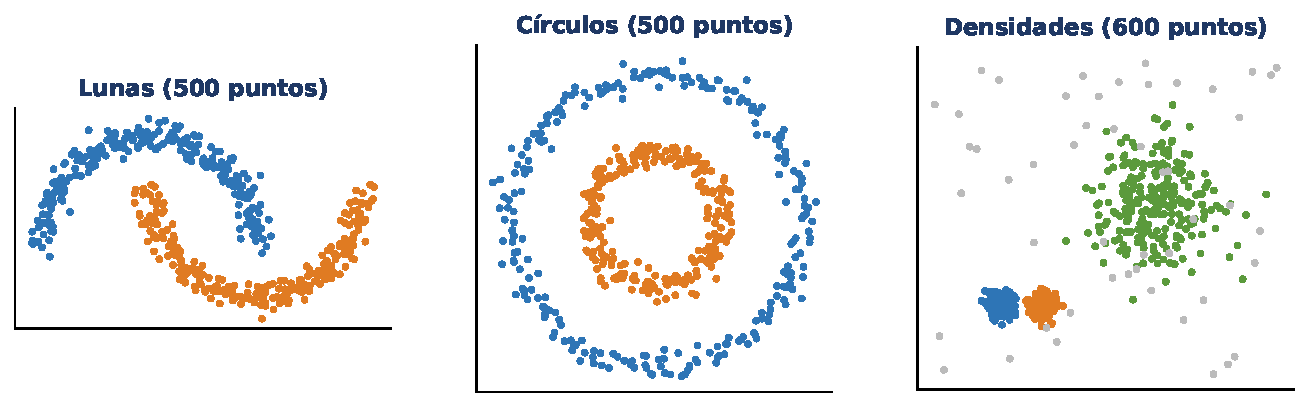
\includegraphics[width=0.95\textwidth]{lab_datos}
  \begin{itemize}
    \item \textbf{Lunas}: dos grupos entrelazados, no convexos.
    \item \textbf{Círculos}: un grupo rodea al otro; ningún centro los separa.
    \item \textbf{Densidades}: dos grupos densos y pegados, uno disperso, y 50 puntos de ruido uniforme.
  \end{itemize}
\end{frame}

\begin{frame}[fragile]{Paso 2: elegir $\eps$ para DBSCAN}
\begin{lstlisting}
for nombre, (X, y) in datos.items():
    d = np.sort(NearestNeighbors(n_neighbors=10).fit(X).kneighbors(X)[0][:, -1])
    plt.plot(d)    # grafica de k-distancia con min_samples = 10
\end{lstlisting}
  \centering
  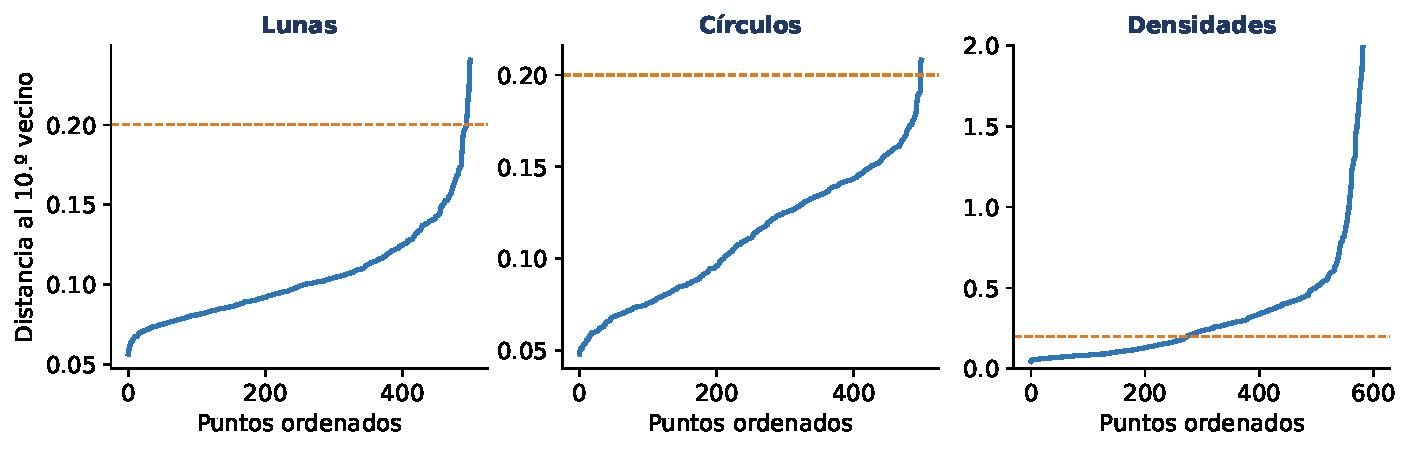
\includegraphics[width=0.9\textwidth]{lab_k_distancia}
  \begin{itemize}
    \item En lunas y círculos el codo está cerca de 0.2: se usa $\eps = 0.2$ y \texttt{min\_samples} $= 10$.
    \item En densidades la curva sube de forma gradual: no hay un codo claro, señal de que las
          densidades son distintas.
  \end{itemize}
\end{frame}

\begin{frame}[fragile]{Paso 3: DBSCAN con densidades distintas}
\begin{lstlisting}
X, y = datos["Densidades"]
for eps in np.arange(0.1, 1.01, 0.05):
    z = DBSCAN(eps=eps, min_samples=10).fit_predict(X)
    print(round(eps, 2), adjusted_rand_score(y, z))
\end{lstlisting}
  \begin{columns}[c]
    \column{0.48\textwidth}
    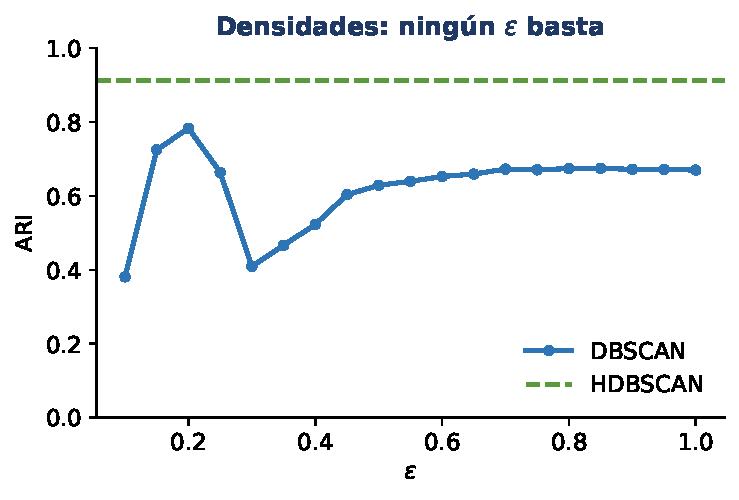
\includegraphics[width=\textwidth]{lab_barrido}
    \column{0.5\textwidth}
    \small
    \begin{itemize}
      \item El mejor DBSCAN obtiene ARI 0.78, con $\eps = 0.2$: separa los dos grupos densos,
            pero 236 de los 250 puntos del disperso quedan como ruido.
      \item Con $\eps \ge 0.35$ los dos densos se unen en un grupo; el disperso aparece, pero con parte de sus puntos como ruido.
      \item HDBSCAN, con \texttt{min\_cluster\_size} $=15$ y sin elegir $\eps$, obtiene 0.91.
    \end{itemize}
  \end{columns}
\end{frame}

\begin{frame}[fragile]{Paso 4: los cuatro métodos en los tres conjuntos}
\begin{lstlisting}
for nombre, (X, y) in datos.items():
    k = len(set(y) - {-1})
    modelos = {"k-medias": KMeans(k, n_init=10, random_state=0),
               "DBSCAN": DBSCAN(eps=0.2, min_samples=10),
               "HDBSCAN": HDBSCAN(min_cluster_size=15),
               "Espectral": SpectralClustering(k, affinity="nearest_neighbors",
                                               n_neighbors=10, random_state=0)}
    for metodo, modelo in modelos.items():
        z = modelo.fit_predict(X)
        print(nombre, metodo, round(adjusted_rand_score(y, z), 2), (z == -1).sum())
\end{lstlisting}
  \vspace{4pt}
  \centering
  \small
  \begin{tabular}{@{}lcccc@{}}
    \toprule
    \textbf{ARI} & \textbf{k-medias} & \textbf{DBSCAN} & \textbf{HDBSCAN} & \textbf{Espectral}\\
    \midrule
    Lunas      & 0.24 & 1.00 & 1.00 & 1.00 \\
    Círculos   & 0.00 & 1.00 & 1.00 & 1.00 \\
    Densidades & 0.46 & 0.78 & 0.91 & 0.85 \\
    \bottomrule
  \end{tabular}
\end{frame}

\begin{frame}{Paso 4: los resultados}
  \begin{columns}[c]
    \column{0.58\textwidth}
    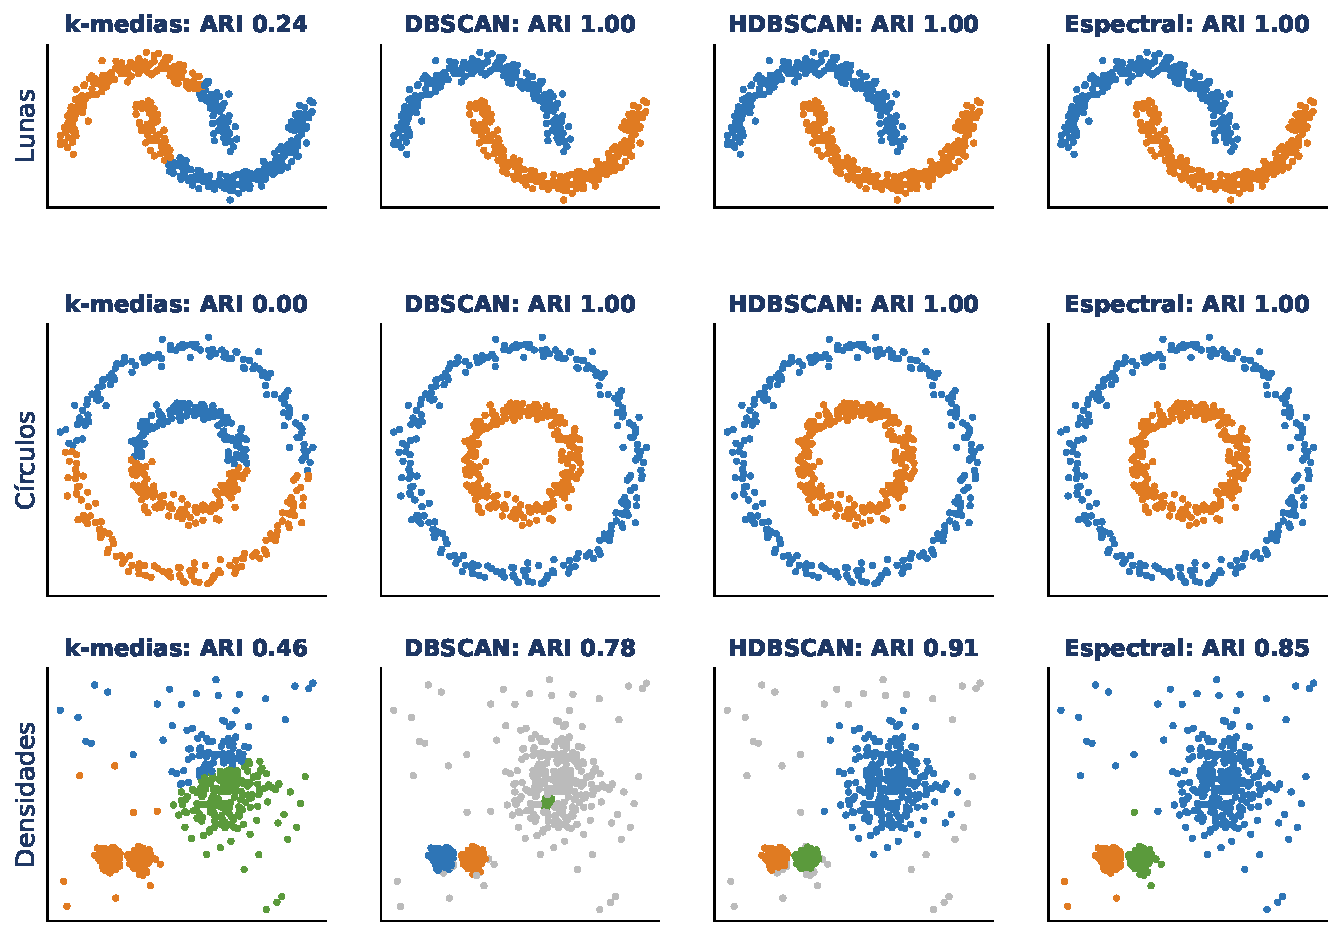
\includegraphics[width=\textwidth]{lab_comparacion}
    \column{0.4\textwidth}
    \small
    \begin{itemize}
      \item Lunas y círculos: los tres métodos no convexos aciertan; k-medias corta las formas.
      \item Densidades, espectral: separa bien los tres grupos, pero asigna los 50 puntos de
            ruido a algún grupo (no tiene etiqueta de ruido).
      \item Densidades, HDBSCAN: marca 47 puntos como ruido; 35 son del ruido inyectado.
            Los otros 15 puntos de ruido quedan junto al grupo disperso y se le asignan.
      \item k-medias divide el grupo disperso y une los dos densos.
    \end{itemize}
  \end{columns}
\end{frame}

\begin{frame}{Conclusiones del laboratorio}
  \begin{itemize}
    \item Con grupos no convexos de densidad parecida (lunas, círculos), DBSCAN, HDBSCAN y espectral
          recuperan los grupos; k-medias no.
    \item La gráfica de k-distancia da un buen $\eps$ cuando tiene un codo claro; si no lo tiene,
          las densidades son distintas y ningún $\eps$ basta.
    \item HDBSCAN resuelve las densidades distintas con un parámetro fácil de interpretar
          (\texttt{min\_cluster\_size}) y además marca el ruido.
    \item El agrupamiento espectral separa bien los grupos, pero necesita $K$ y no detecta ruido.
    \item Los mismos parámetros ($\eps=0.2$, \texttt{min\_samples} $=10$, \texttt{min\_cluster\_size} $=15$,
          10 vecinos) sirvieron en los tres conjuntos porque tienen escalas parecidas; con otros
          datos hay que estandarizar y volver a elegirlos.
  \end{itemize}
\end{frame}

%  El mismo código, ejecutado, está en laboratorio_densidad_espectral.ipynb
% =====================================================================
\section{Laboratorio: densidad y espectral en formas no convexas}
% =====================================================================

\begin{frame}[fragile]{Paso 1: los datos}
\begin{lstlisting}
import numpy as np, pandas as pd
from sklearn.datasets import make_moons, make_circles, make_blobs
from sklearn.cluster import KMeans, DBSCAN, HDBSCAN, SpectralClustering
from sklearn.neighbors import NearestNeighbors
from sklearn.metrics import adjusted_rand_score

Xm, ym = make_moons(500, noise=0.07, random_state=0)
Xc, yc = make_circles(500, factor=0.45, noise=0.05, random_state=0)
Xb, yb = make_blobs([150, 150, 250], centers=[[0, 0], [1.3, 0], [4.5, 3]],
                    cluster_std=[0.2, 0.2, 1.0], random_state=0)
ruido = np.random.default_rng(0).uniform([-2, -2], [8, 7], (50, 2))
Xd, yd = np.r_[Xb, ruido], np.r_[yb, -np.ones(50, int)]   # el ruido tiene etiqueta -1
datos = {"Lunas": (Xm, ym), "Círculos": (Xc, yc), "Densidades": (Xd, yd)}
\end{lstlisting}
  {\small Las etiquetas verdaderas sólo se usan para evaluar con el ARI; el ruido cuenta como una clase más.}
\end{frame}

\begin{frame}{Paso 1: los tres conjuntos}
  \centering
  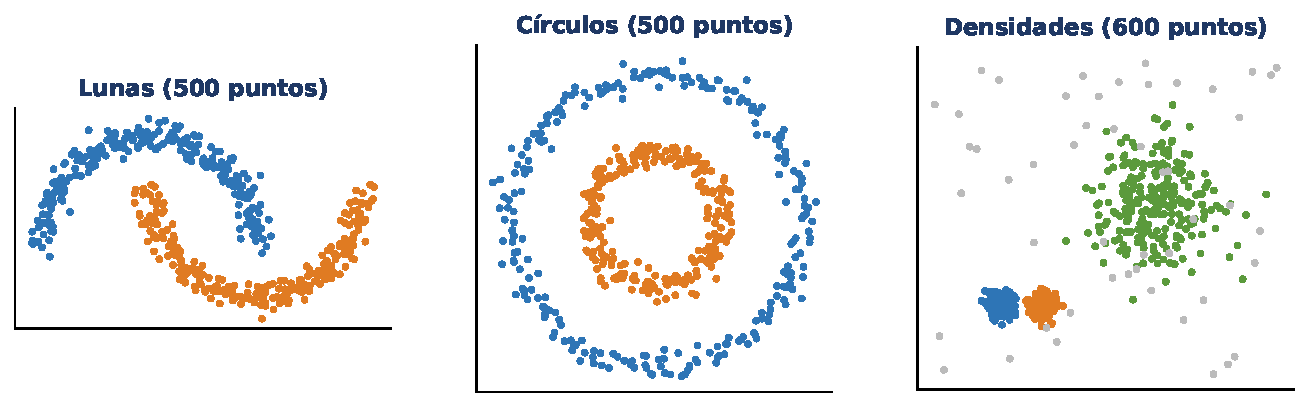
\includegraphics[width=0.95\textwidth]{lab_datos}
  \begin{itemize}
    \item \textbf{Lunas}: dos grupos entrelazados, no convexos.
    \item \textbf{Círculos}: un grupo rodea al otro; ningún centro los separa.
    \item \textbf{Densidades}: dos grupos densos y pegados, uno disperso, y 50 puntos de ruido uniforme.
  \end{itemize}
\end{frame}

\begin{frame}[fragile]{Paso 2: elegir $\eps$ para DBSCAN}
\begin{lstlisting}
for nombre, (X, y) in datos.items():
    d = np.sort(NearestNeighbors(n_neighbors=10).fit(X).kneighbors(X)[0][:, -1])
    plt.plot(d)    # grafica de k-distancia con min_samples = 10
\end{lstlisting}
  \centering
  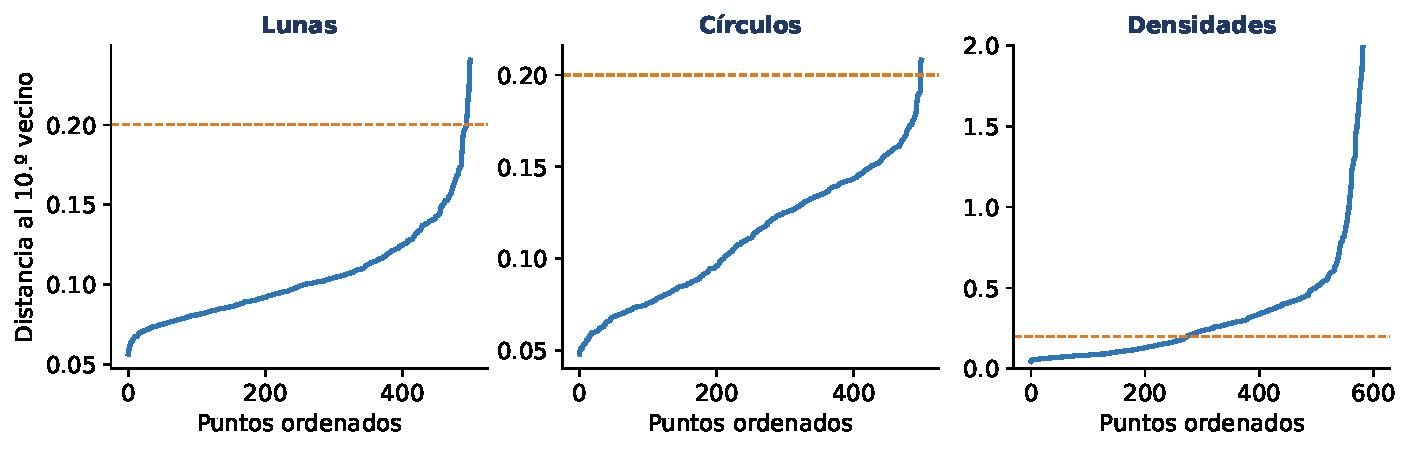
\includegraphics[width=0.9\textwidth]{lab_k_distancia}
  \begin{itemize}
    \item En lunas y círculos el codo está cerca de 0.2: se usa $\eps = 0.2$ y \texttt{min\_samples} $= 10$.
    \item En densidades la curva sube de forma gradual: no hay un codo claro, señal de que las
          densidades son distintas.
  \end{itemize}
\end{frame}

\begin{frame}[fragile]{Paso 3: DBSCAN con densidades distintas}
\begin{lstlisting}
X, y = datos["Densidades"]
for eps in np.arange(0.1, 1.01, 0.05):
    z = DBSCAN(eps=eps, min_samples=10).fit_predict(X)
    print(round(eps, 2), adjusted_rand_score(y, z))
\end{lstlisting}
  \begin{columns}[c]
    \column{0.48\textwidth}
    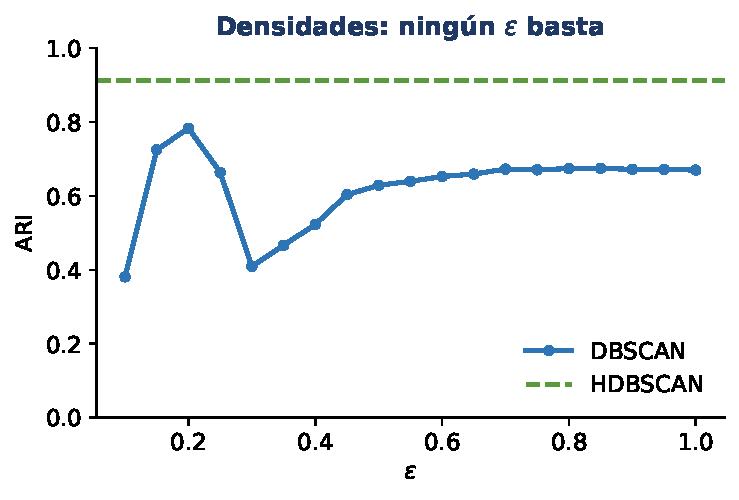
\includegraphics[width=\textwidth]{lab_barrido}
    \column{0.5\textwidth}
    \small
    \begin{itemize}
      \item El mejor DBSCAN obtiene ARI 0.78, con $\eps = 0.2$: separa los dos grupos densos,
            pero 236 de los 250 puntos del disperso quedan como ruido.
      \item Con $\eps \ge 0.35$ los dos densos se unen en un grupo; el disperso aparece, pero con parte de sus puntos como ruido.
      \item HDBSCAN, con \texttt{min\_cluster\_size} $=15$ y sin elegir $\eps$, obtiene 0.91.
    \end{itemize}
  \end{columns}
\end{frame}

\begin{frame}[fragile]{Paso 4: los cuatro métodos en los tres conjuntos}
\begin{lstlisting}
for nombre, (X, y) in datos.items():
    k = len(set(y) - {-1})
    modelos = {"k-medias": KMeans(k, n_init=10, random_state=0),
               "DBSCAN": DBSCAN(eps=0.2, min_samples=10),
               "HDBSCAN": HDBSCAN(min_cluster_size=15),
               "Espectral": SpectralClustering(k, affinity="nearest_neighbors",
                                               n_neighbors=10, random_state=0)}
    for metodo, modelo in modelos.items():
        z = modelo.fit_predict(X)
        print(nombre, metodo, round(adjusted_rand_score(y, z), 2), (z == -1).sum())
\end{lstlisting}
  \vspace{4pt}
  \centering
  \small
  \begin{tabular}{@{}lcccc@{}}
    \toprule
    \textbf{ARI} & \textbf{k-medias} & \textbf{DBSCAN} & \textbf{HDBSCAN} & \textbf{Espectral}\\
    \midrule
    Lunas      & 0.24 & 1.00 & 1.00 & 1.00 \\
    Círculos   & 0.00 & 1.00 & 1.00 & 1.00 \\
    Densidades & 0.46 & 0.78 & 0.91 & 0.85 \\
    \bottomrule
  \end{tabular}
\end{frame}

\begin{frame}{Paso 4: los resultados}
  \begin{columns}[c]
    \column{0.58\textwidth}
    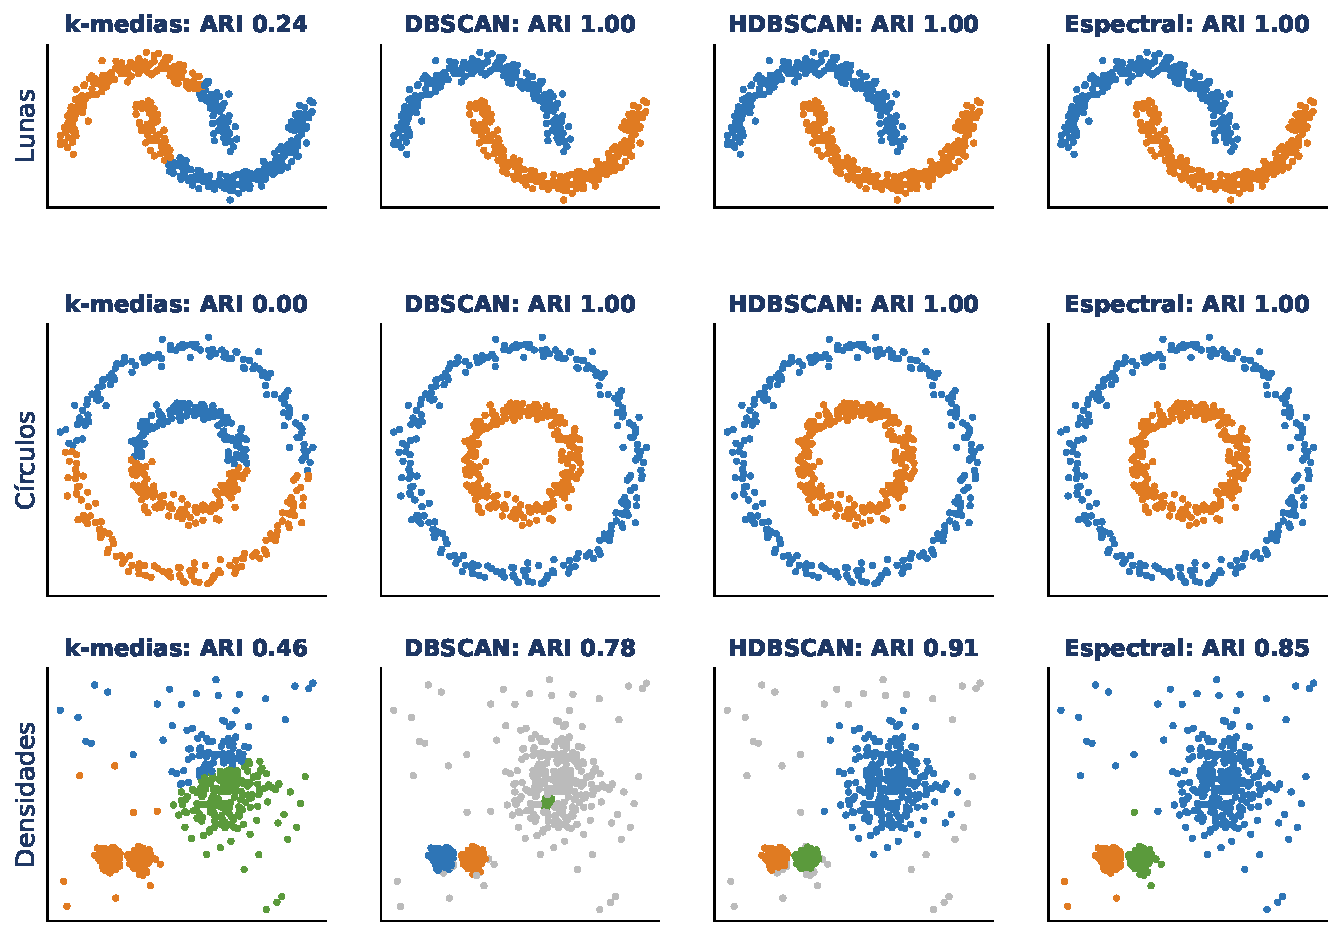
\includegraphics[width=\textwidth]{lab_comparacion}
    \column{0.4\textwidth}
    \small
    \begin{itemize}
      \item Lunas y círculos: los tres métodos no convexos aciertan; k-medias corta las formas.
      \item Densidades, espectral: separa bien los tres grupos, pero asigna los 50 puntos de
            ruido a algún grupo (no tiene etiqueta de ruido).
      \item Densidades, HDBSCAN: marca 47 puntos como ruido; 35 son del ruido inyectado.
            Los otros 15 puntos de ruido quedan junto al grupo disperso y se le asignan.
      \item k-medias divide el grupo disperso y une los dos densos.
    \end{itemize}
  \end{columns}
\end{frame}

\begin{frame}{Conclusiones del laboratorio}
  \begin{itemize}
    \item Con grupos no convexos de densidad parecida (lunas, círculos), DBSCAN, HDBSCAN y espectral
          recuperan los grupos; k-medias no.
    \item La gráfica de k-distancia da un buen $\eps$ cuando tiene un codo claro; si no lo tiene,
          las densidades son distintas y ningún $\eps$ basta.
    \item HDBSCAN resuelve las densidades distintas con un parámetro fácil de interpretar
          (\texttt{min\_cluster\_size}) y además marca el ruido.
    \item El agrupamiento espectral separa bien los grupos, pero necesita $K$ y no detecta ruido.
    \item Los mismos parámetros ($\eps=0.2$, \texttt{min\_samples} $=10$, \texttt{min\_cluster\_size} $=15$,
          10 vecinos) sirvieron en los tres conjuntos porque tienen escalas parecidas; con otros
          datos hay que estandarizar y volver a elegirlos.
  \end{itemize}
\end{frame}

%  El mismo código, ejecutado, está en laboratorio_densidad_espectral.ipynb
% =====================================================================
\section{Laboratorio: densidad y espectral en formas no convexas}
% =====================================================================

\begin{frame}[fragile]{Paso 1: los datos}
\begin{lstlisting}
import numpy as np, pandas as pd
from sklearn.datasets import make_moons, make_circles, make_blobs
from sklearn.cluster import KMeans, DBSCAN, HDBSCAN, SpectralClustering
from sklearn.neighbors import NearestNeighbors
from sklearn.metrics import adjusted_rand_score

Xm, ym = make_moons(500, noise=0.07, random_state=0)
Xc, yc = make_circles(500, factor=0.45, noise=0.05, random_state=0)
Xb, yb = make_blobs([150, 150, 250], centers=[[0, 0], [1.3, 0], [4.5, 3]],
                    cluster_std=[0.2, 0.2, 1.0], random_state=0)
ruido = np.random.default_rng(0).uniform([-2, -2], [8, 7], (50, 2))
Xd, yd = np.r_[Xb, ruido], np.r_[yb, -np.ones(50, int)]   # el ruido tiene etiqueta -1
datos = {"Lunas": (Xm, ym), "Círculos": (Xc, yc), "Densidades": (Xd, yd)}
\end{lstlisting}
  {\small Las etiquetas verdaderas sólo se usan para evaluar con el ARI; el ruido cuenta como una clase más.}
\end{frame}

\begin{frame}{Paso 1: los tres conjuntos}
  \centering
  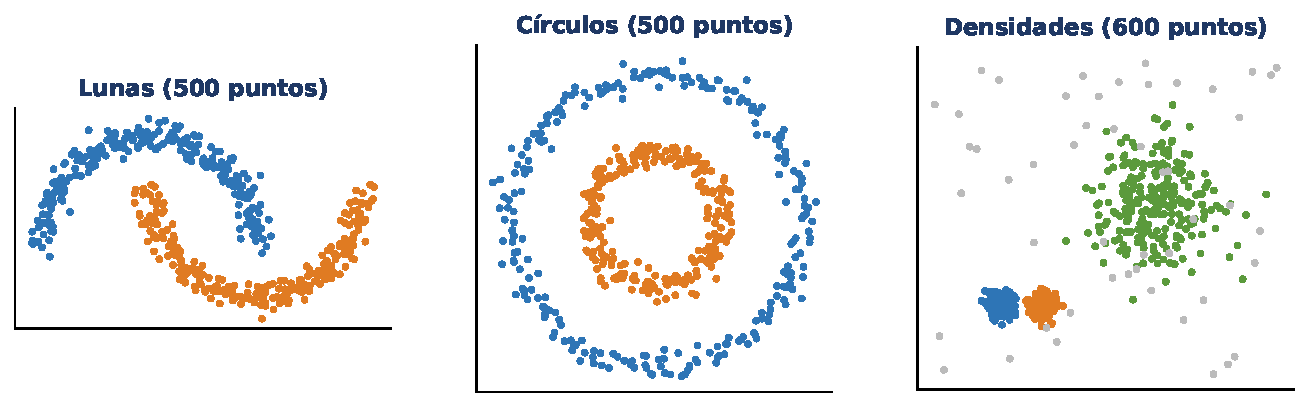
\includegraphics[width=0.95\textwidth]{lab_datos}
  \begin{itemize}
    \item \textbf{Lunas}: dos grupos entrelazados, no convexos.
    \item \textbf{Círculos}: un grupo rodea al otro; ningún centro los separa.
    \item \textbf{Densidades}: dos grupos densos y pegados, uno disperso, y 50 puntos de ruido uniforme.
  \end{itemize}
\end{frame}

\begin{frame}[fragile]{Paso 2: elegir $\eps$ para DBSCAN}
\begin{lstlisting}
for nombre, (X, y) in datos.items():
    d = np.sort(NearestNeighbors(n_neighbors=10).fit(X).kneighbors(X)[0][:, -1])
    plt.plot(d)    # grafica de k-distancia con min_samples = 10
\end{lstlisting}
  \centering
  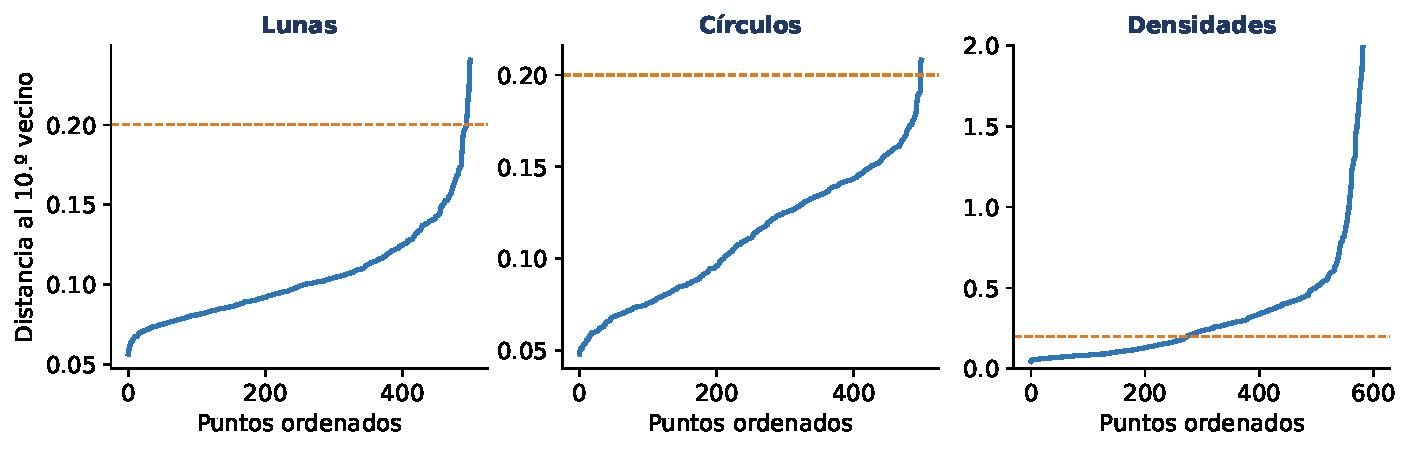
\includegraphics[width=0.9\textwidth]{lab_k_distancia}
  \begin{itemize}
    \item En lunas y círculos el codo está cerca de 0.2: se usa $\eps = 0.2$ y \texttt{min\_samples} $= 10$.
    \item En densidades la curva sube de forma gradual: no hay un codo claro, señal de que las
          densidades son distintas.
  \end{itemize}
\end{frame}

\begin{frame}[fragile]{Paso 3: DBSCAN con densidades distintas}
\begin{lstlisting}
X, y = datos["Densidades"]
for eps in np.arange(0.1, 1.01, 0.05):
    z = DBSCAN(eps=eps, min_samples=10).fit_predict(X)
    print(round(eps, 2), adjusted_rand_score(y, z))
\end{lstlisting}
  \begin{columns}[c]
    \column{0.48\textwidth}
    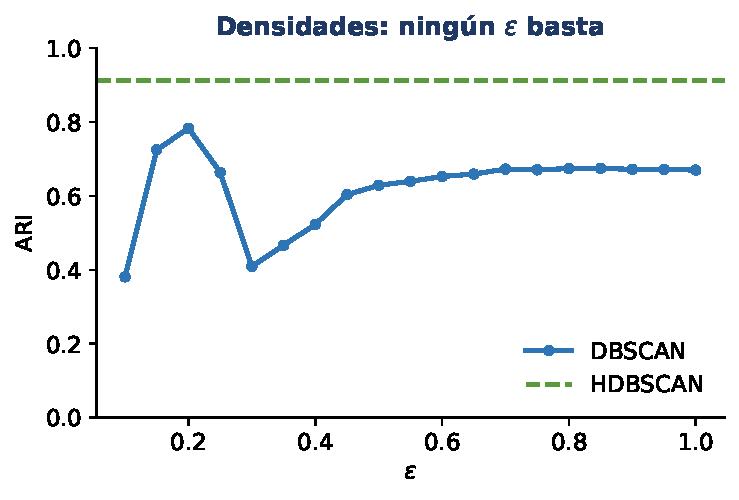
\includegraphics[width=\textwidth]{lab_barrido}
    \column{0.5\textwidth}
    \small
    \begin{itemize}
      \item El mejor DBSCAN obtiene ARI 0.78, con $\eps = 0.2$: separa los dos grupos densos,
            pero 236 de los 250 puntos del disperso quedan como ruido.
      \item Con $\eps \ge 0.35$ los dos densos se unen en un grupo; el disperso aparece, pero con parte de sus puntos como ruido.
      \item HDBSCAN, con \texttt{min\_cluster\_size} $=15$ y sin elegir $\eps$, obtiene 0.91.
    \end{itemize}
  \end{columns}
\end{frame}

\begin{frame}[fragile]{Paso 4: los cuatro métodos en los tres conjuntos}
\begin{lstlisting}
for nombre, (X, y) in datos.items():
    k = len(set(y) - {-1})
    modelos = {"k-medias": KMeans(k, n_init=10, random_state=0),
               "DBSCAN": DBSCAN(eps=0.2, min_samples=10),
               "HDBSCAN": HDBSCAN(min_cluster_size=15),
               "Espectral": SpectralClustering(k, affinity="nearest_neighbors",
                                               n_neighbors=10, random_state=0)}
    for metodo, modelo in modelos.items():
        z = modelo.fit_predict(X)
        print(nombre, metodo, round(adjusted_rand_score(y, z), 2), (z == -1).sum())
\end{lstlisting}
  \vspace{4pt}
  \centering
  \small
  \begin{tabular}{@{}lcccc@{}}
    \toprule
    \textbf{ARI} & \textbf{k-medias} & \textbf{DBSCAN} & \textbf{HDBSCAN} & \textbf{Espectral}\\
    \midrule
    Lunas      & 0.24 & 1.00 & 1.00 & 1.00 \\
    Círculos   & 0.00 & 1.00 & 1.00 & 1.00 \\
    Densidades & 0.46 & 0.78 & 0.91 & 0.85 \\
    \bottomrule
  \end{tabular}
\end{frame}

\begin{frame}{Paso 4: los resultados}
  \begin{columns}[c]
    \column{0.58\textwidth}
    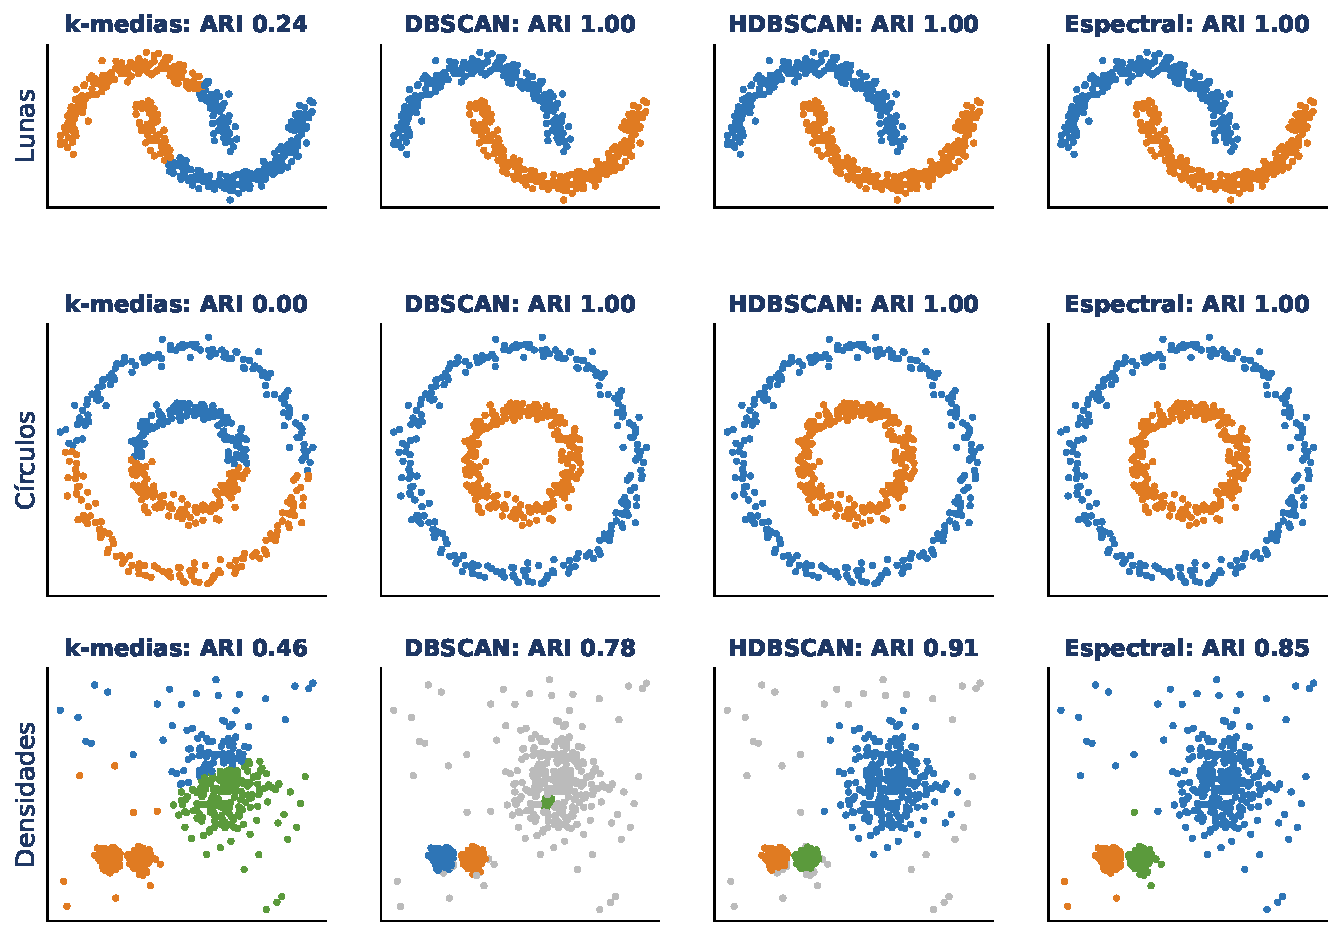
\includegraphics[width=\textwidth]{lab_comparacion}
    \column{0.4\textwidth}
    \small
    \begin{itemize}
      \item Lunas y círculos: los tres métodos no convexos aciertan; k-medias corta las formas.
      \item Densidades, espectral: separa bien los tres grupos, pero asigna los 50 puntos de
            ruido a algún grupo (no tiene etiqueta de ruido).
      \item Densidades, HDBSCAN: marca 47 puntos como ruido; 35 son del ruido inyectado.
            Los otros 15 puntos de ruido quedan junto al grupo disperso y se le asignan.
      \item k-medias divide el grupo disperso y une los dos densos.
    \end{itemize}
  \end{columns}
\end{frame}

\begin{frame}{Conclusiones del laboratorio}
  \begin{itemize}
    \item Con grupos no convexos de densidad parecida (lunas, círculos), DBSCAN, HDBSCAN y espectral
          recuperan los grupos; k-medias no.
    \item La gráfica de k-distancia da un buen $\eps$ cuando tiene un codo claro; si no lo tiene,
          las densidades son distintas y ningún $\eps$ basta.
    \item HDBSCAN resuelve las densidades distintas con un parámetro fácil de interpretar
          (\texttt{min\_cluster\_size}) y además marca el ruido.
    \item El agrupamiento espectral separa bien los grupos, pero necesita $K$ y no detecta ruido.
    \item Los mismos parámetros ($\eps=0.2$, \texttt{min\_samples} $=10$, \texttt{min\_cluster\_size} $=15$,
          10 vecinos) sirvieron en los tres conjuntos porque tienen escalas parecidas; con otros
          datos hay que estandarizar y volver a elegirlos.
  \end{itemize}
\end{frame}

% =====================================================================

\begin{frame}{Resumen}
  \begin{itemize}
    \item Los métodos por densidad definen un grupo como una región densa; no suponen formas convexas.
    \item DBSCAN clasifica los puntos en núcleo, frontera y ruido con $\eps$ y \texttt{min\_samples};
          $\eps$ se elige con la gráfica de k-distancia.
    \item Un solo $\eps$ falla con densidades distintas: OPTICS muestra todas las escalas y HDBSCAN
          elige cada grupo a su propia escala.
    \item El agrupamiento espectral agrupa los nodos de un grafo de similitud con los vectores propios
          del laplaciano; necesita $K$ y no detecta ruido.
  \end{itemize}
  \vspace{6pt}
  \begin{block}{Próxima sesión}
    Validación e interpretación de agrupamientos.
  \end{block}
\end{frame}

\end{document}
